\apendice{Documentación de usuario}

\section{Introducción}
En esta sección, nos vamos a centrar en explicar y mostrar paso a paso, como un usuario puede llegar a usar esta aplicación de forma intuitiva y sencilla.
\section{Requisitos de usuarios}
Para que un usuario pueda ejecutar y usar nuestra aplicación, deberá tener instalado Python 3.5 en su maquina, aunque para facilitar al usuario no tener que saber como descargar las librerías o dependencias, hemos implementado un script que funcionara teniendo instalado Miniconda para Python 3.5, explicaremos su uso en la instalación.

\begin{itemize}
	\item Tener una distribución Windows instalada.

	\item Python 3.5: Para poder ejecutar necesitaremos tener Python 3.5.
	\begin{itemize}
		\item Miniconda para Python 3.5:
		
		Se puede descargar a través del siguiente enlace \url{http://conda.pydata.org/miniconda.html} y siguiendo las instrucciones a traves de este otro enlace \url{http://conda.pydata.org/docs/install/quick.html#windows-miniconda-install}.		
		
		Es una distribución que incluye Python y facilita el uso de este lenguaje y la instalación de multitud de librerías.
		
		Sera necesario tenerlo instalado en la carpeta principal de nuestro usuario C:\textbackslash Users\textbackslash NombreTuUsuario
	\end{itemize}
	
	\item Tener el proyecto descargado o clonado con los fuentes:
	
	Se puede descargar a través del siguiente enlace \url{https://github.com/Itg0001/TFG_DietaPorDientes.git}

\end{itemize}

\section{Instalación}

Una vez que tengamos Miniconda para Python 3.5 y el proyecto descargado o clonado podremos proceder a la instalación del mismo, siguiendo los pasos descritos a continuación:

\begin{itemize}
	\item Primero si hemos descargado el proyecto lo tendremos en formato .zip deberemos descomprimirlo en la carpeta deseada.
	
	\item Una vez descomprimido dentro del fichero del proyecto estará ubicado un ejecutable para Windows .bat llamado <<EjecutarGui.bat>>.
	
	Procederemos a hacer doble clic sobre este fichero ejecutable y se abrirá una terminal, la primera vez que lo hagamos este proceso tardara un rato, porque descarga las librerías necesarias para la ejecución del mismo.
	
	\item Una vez terminado el proceso anterior, se abrira la aplicación.
\end{itemize}

\subsection{Cuando algo falla}
En caso de que al instalar o descargar los paquetes salta algún error esto se deberá a que se habrá perdido la conexión a Internet y no puede descargar los paquetes necesarios.
Para solucionarlo volvemos a ejecutar y comenzara donde se quedo al caerse la red. No perdemos el tiempo usado hasta ese momento.

Otro fallo común es que no se haya instalado la distribución de Miniconda sobre el directorio indicado: C:\textbackslash Users\textbackslash NombreTuUsuario.
Para solucionar este problema deberemos instalarlo sobre este directorio.

En caso de que surja algún otro problema contactar con el desarrollador a través del siguiente EMAIL: itg0001\makeatletter @ alu.ubu.es 

\section{Manual del usuario}

Una vez tengamos todo bien configurado y la aplicación ejecute correctamente deberíamos tener esta ventana inicial.

\begin{figure}[h]
\centering
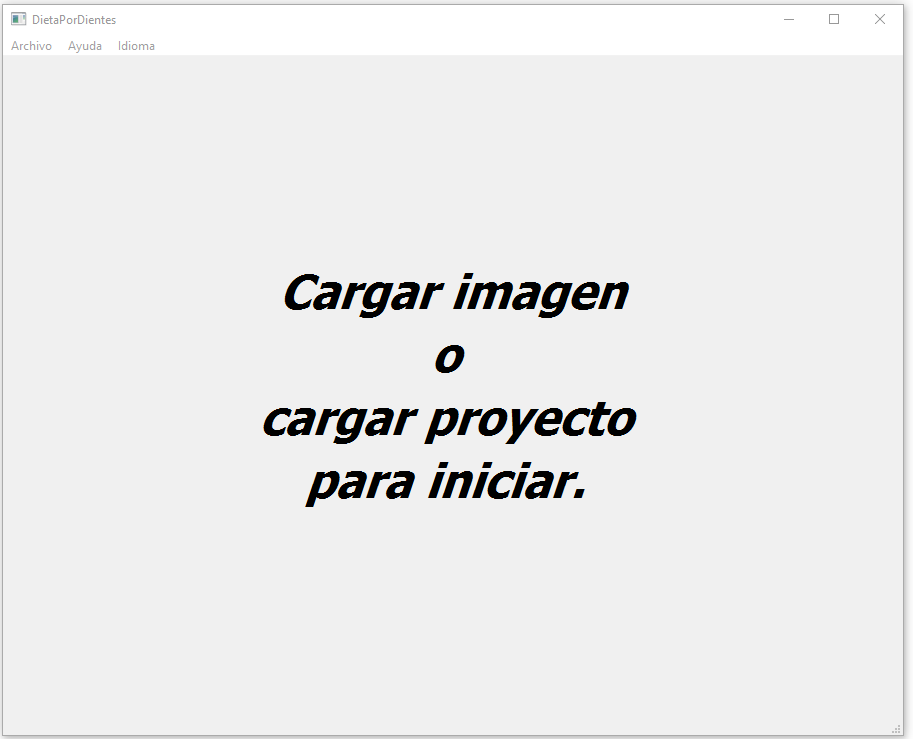
\includegraphics[width=.99\textwidth]{VentanaInicial}
\caption{Ventana inicial de la aplicación}
\label{fig:E.1}
\end{figure}
Una vez llegados a este punto tendremos varias opciones para editar o calculas las estrias de una imagen, dependiendo si esta en blanco o ya pintada tendremos las siguientes opciones:

\begin{itemize}
	\item Abrir imagen \ref{modo:1}:

	\item Cargar proyecto \ref{modo:2}:
	
	\item[Modo 1] Semiautomatico  \ref{modo:2.1}
	\item[Modo 2] Manual \ref{modo:2.2}
	\item[Modo 3] Automatico \ref{modo:2.3}
\end{itemize}


\label{modo:1}
\subsection{Abrir imagen}
En esta sección se explicara como cargar una imagen en nuestra aplicación, para empezar un proyecto desde cero.

Deberemos seleccionar la opción de Archivo  $>$ Nuevo Proyecto. Como se puede ver en la imagen \ref{fig:abrirPro}

\begin{figure}[h]
\centering
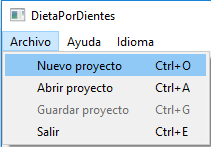
\includegraphics[width=.50\textwidth]{AbrirImagen}
\caption{Opción para cargar una imagen}
\label{fig:abrirPro}
\end{figure}

Una vez que clicamos en este punto se nos muestra una ventana de elegir ficheros en el cual debemos explorar hasta la carpeta donde estén las imágenes que queremos analizar. Como podemos observar en la figura \ref{fig:abrirPaso2}

\begin{figure}[h]
\centering
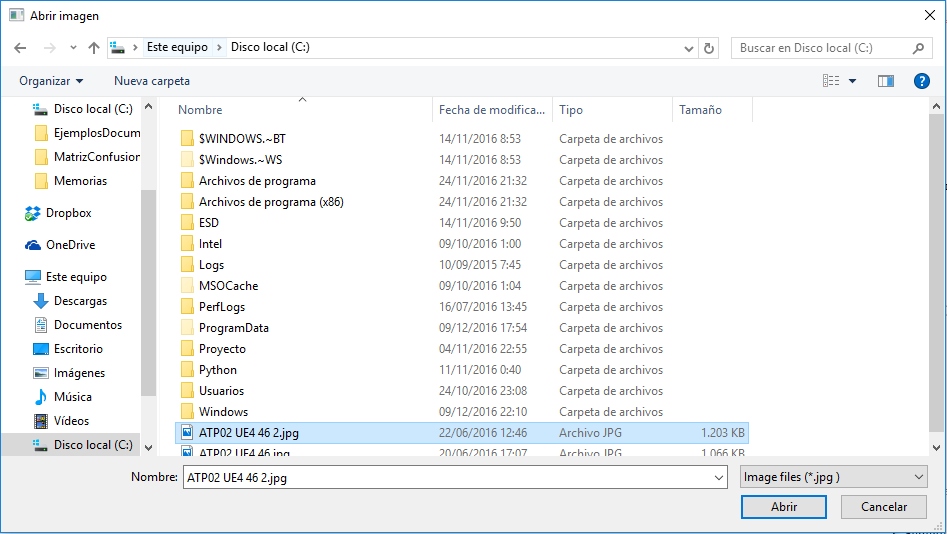
\includegraphics[width=.99\textwidth]{AbrirPaso2}
\caption{Seleccionador de ficheros}
\label{fig:abrirPaso2}
\end{figure}

Una vez seleccionado deberemos dar a aceptar si hemos seleccionado la imagen que queremos evaluar.
Dependiendo de la imagen que hemos abierto pueden pasar dos cosas, uno \ref{fig:opcion1}, que la imagen abierta este pintada, dos \ref{fig:opcion2}, que la imagen abierta no este pintada. Dependiendo de esto tendremos estas dos ventanas, como se muestra en la figura.


\begin{figure}
	\begin{subfigure}[c]{.5\linewidth}
	\centering\large 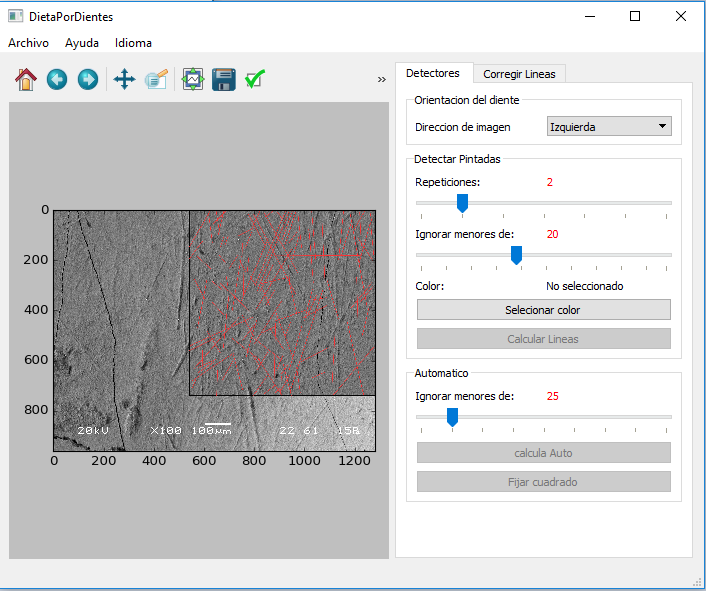
\includegraphics[width=.9\textwidth]{opcion1}
	\caption{Opcion con lineas pintadas.}\label{fig:opcion1}
	\end{subfigure}%
	\begin{subfigure}[c]{.5\linewidth}
	\centering\large 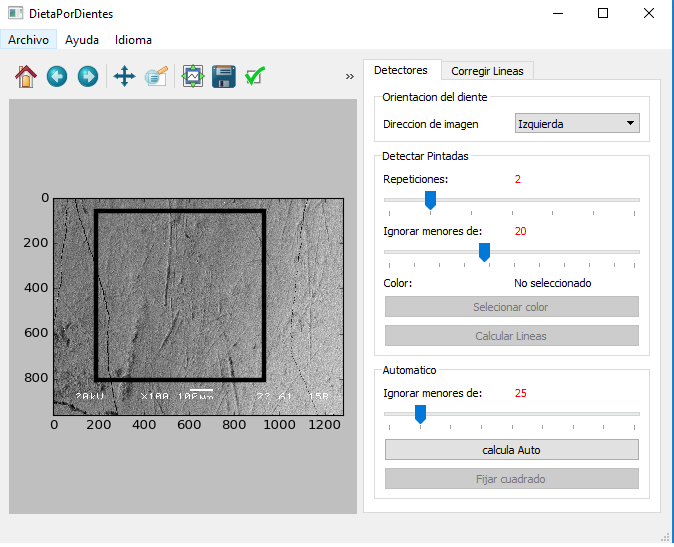
\includegraphics[width=.9\textwidth]{opcion2}
	\caption{Opcion con lineas sin pintar.}\label{fig:opcion2}
	\end{subfigure}%
\end{figure}




\label{modo:2}
\subsection{Cargar proyecto}
En esta sección se explicara como cargar un proyecto en nuestra aplicación, para continuar un proyecto ya empezado.

Deberemos seleccionar la opción de Archivo  $>$ Abrir Proyecto. Como se puede ver en la figura \ref{fig:cargarPro}


\begin{figure}[h]
\centering
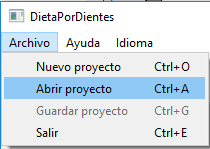
\includegraphics[width=.50\textwidth]{CargarProyecto}
\caption{Opción para abrir un proyecto.}
\label{fig:cargarPro}
\end{figure}

Una vez que hacemos clic sobre la opción anteriormente mencionada ahora debemos seleccionar la carpeta donde estará contenido todos los ficheros del proyecto, como podemos observar en la siguiente figura \ref{fig:selecCargarPro}. y una vez seleccionado el directorio que contiene los ficheros del proyecto damos a <<Abrir carpeta>> para cargar el proyecto. 



\begin{figure}[h]
\centering
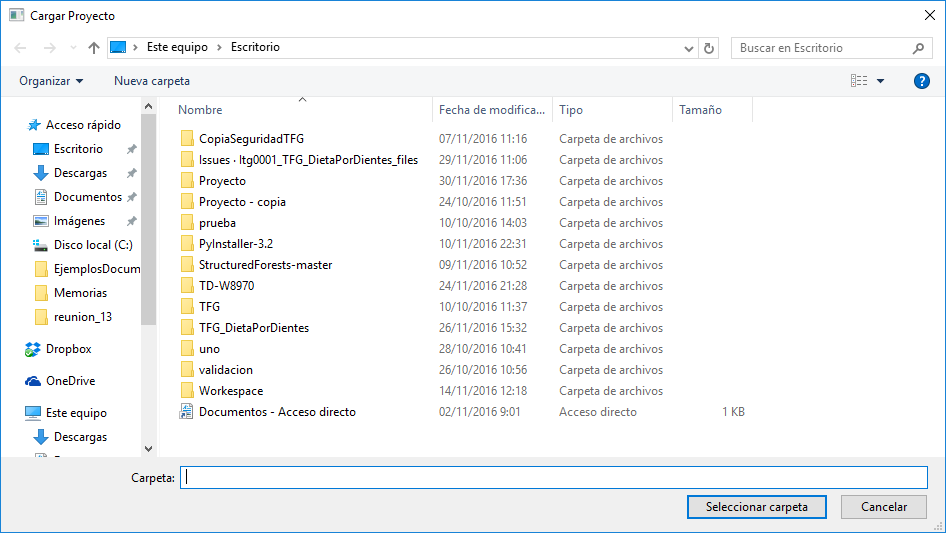
\includegraphics[width=.99\textwidth]{selecCargarPro}
\caption{Opción para abrir un proyecto.}
\label{fig:selecCargarPro}
\end{figure}

Una vez abierto el proyecto tendremos la imagen en blanco y negro junto con sus estrías guardadas que estarán pintadas sobre la imagen, como podemos observar en la figura \ref{fig:proyectoAbierto}.


\begin{figure}[h]
\centering
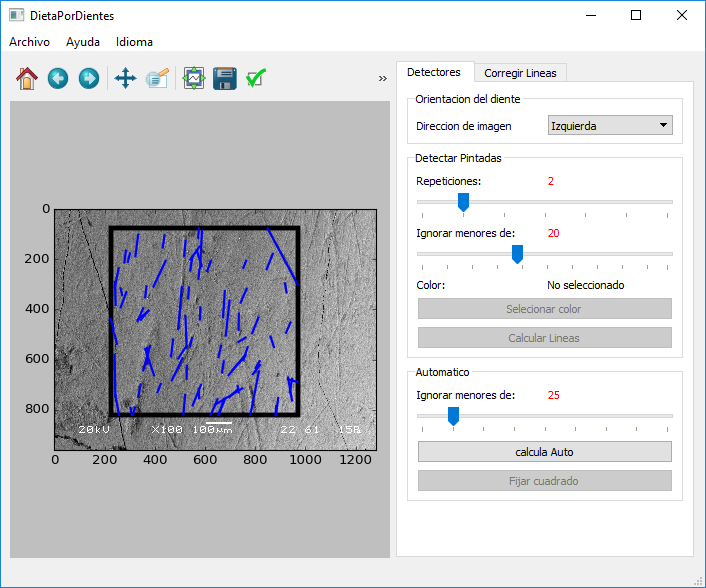
\includegraphics[width=.99\textwidth]{proyectoAbierto}
\caption{Como se muestra un proyecto cargado o abierto.}
\label{fig:proyectoAbierto}
\end{figure}

\label{modo:idioma}
\subsection{Cambiar idioma}
Para cambiar el idioma de la aplicación deberemos seleccionar en el menú principal Idioma $>$ Una de las dos opciones, como podemos obserbar en la figura \ref{cambiarIdioma}, hemos optado por cambiar el idioma de la aplicación y que perduren los cambios realizados en el fichero de configuración por lo que nos va a pedir reiniciar la aplicación, si tenemos algo abierto nos preguntara si queremos guardar los cambios o no.

\begin{figure}[h]
\centering
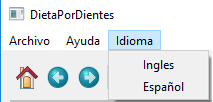
\includegraphics[width=.55\textwidth]{CambiarIdioma}
\caption{Como cambiar el idioma.}
\label{fig:cambiarIdioma}
\end{figure}

\subsection{Modo semi-automático para lineas pintadas}

Este modo solamente podrá ser usado cuando dispongamos de una imagen que tenga las estrías pintadas sobre ella y estas estén contenidas dentro de un cuadrado que delimite su área, como podemos observar en la figura \ref{fig:semiAutoCorrecto}.



\begin{figure}[h]
\centering
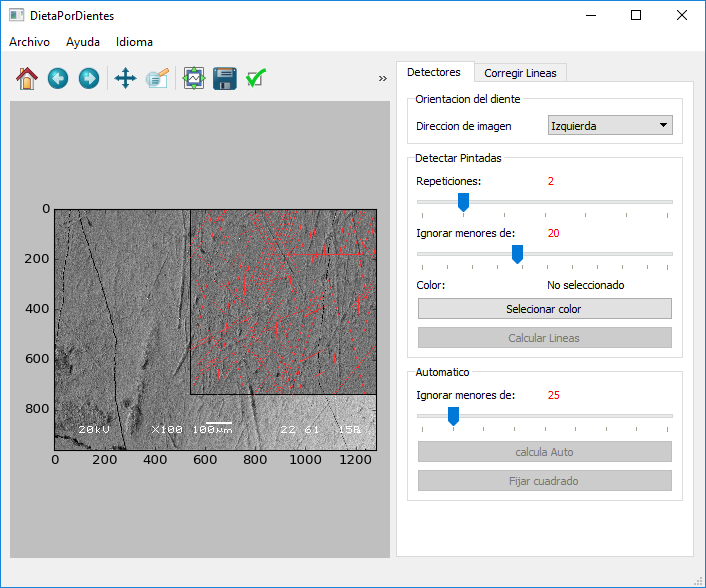
\includegraphics[width=.99\textwidth]{semiAutoCorrecto}
\caption{Imagen valida para detección de estrías modo semi automático.}
\label{fig:semiAutoCorrecto}
\end{figure}

Una vez que tengamos una imagen con las estrías pintadas cargada y valida como mostramos en la figura, procederemos a seleccionar su orientación, como muestra en la siguiente figura \ref{fig:selOrientacion}.

\begin{figure}[h]
\centering
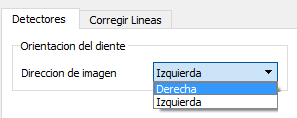
\includegraphics[width=.55\textwidth]{selOrientacion}
\caption{Selección de la orientación de la imagen.}
\label{fig:selOrientacion}
\end{figure}

A continuación deberemos seleccionar tanto el numero de repeticiones del algoritmo para la obtención de los segmentos pintados <<Cuanto mayor número de ellos mas tiempo tardara>>, la longitud mínima que debe ignorar el algoritmo para no detectar segmentos muy pequeños. Como podemos observar en la figura \ref{fig:opcionesAlg}.

\begin{figure}[h]
\centering
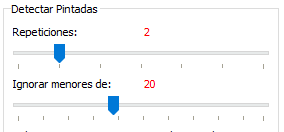
\includegraphics[width=.55\textwidth]{opcionesAlg}
\caption{Selección de las opciones disponibles para este modo.}
\label{fig:opcionesAlg}
\end{figure}

Finalmente para nos quedaría la opción mas importante que sin ella el algoritmo no podrá ser ejecutado. Es seleccionar el color del que estén pintadas las lineas, para ello deberemos clicar sobre el botón <<Seleccionar color>>, como podemos observar en la figura \ref{fig:selecionarColorP1} y despues de clicar sobre el este se desactivara como podemos observar en la figura \ref{fig:selecionarColorP2}.
Las estrías pintadas aveces pueden ser muy finas y no seremos capaces de clicar sobre esos pixeles por lo que en este caso deberemos ampliar la imagen en una región que contenga estrías pintadas, para ampliar debemos seleccionar el botón de ampliar y dibujar un rectángulo sobre la imagen con el clic derecho pulsado,como podemos observar en la figura \ref{fig:selecionarColorP3}.
Una vez seleccionado el color correctamente este pintada el label de color actual y también se activara el botón de calcular las lineas, como podemos observar en la figura \ref{fig:selecionarColorP4}.



\begin{figure}
	\begin{subfigure}[c]{.5\linewidth}
	\centering\large 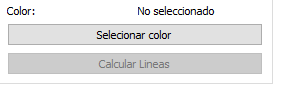
\includegraphics[width=.9\textwidth]{selecionarColorP1}
	\caption{Selección del color en el que estén las estrías pintadas.}\label{fig:selecionarColorP1}
	\end{subfigure}%
	\begin{subfigure}[c]{.5\linewidth}
	\centering\large 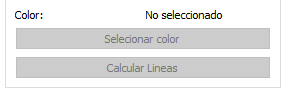
\includegraphics[width=.9\textwidth]{selecionarColorP2}
	\caption{Después de clicar sobre el.}
	\label{fig:selecionarColorP2}
	\end{subfigure}%
	
	\begin{subfigure}[c]{.5\linewidth}
	\centering\large 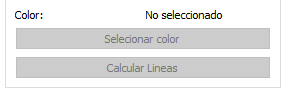
\includegraphics[width=.9\textwidth]{selecionarColorP2}
	\caption{Ampliar región.}
	\label{fig:selecionarColorP3}
	\end{subfigure}%
	\begin{subfigure}[c]{.5\linewidth}
	\centering\large 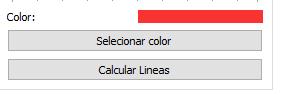
\includegraphics[width=.9\textwidth]{selecionarColorP4}
	\caption{Después de seleccionar correctamente el color.}
	\label{fig:selecionarColorP4}
	\end{subfigure}%
\end{figure}




\label{modo:2.1}
\subsubsection{Modo Semiautomatico}

\label{modo:2.2}
\subsubsection{Modo Manual}

\label{modo:2.3}
\subsubsection{Modo Automatico}







